\documentclass[a4paper]{article}
\usepackage{epsfig,epic,eepic,amssymb}
\graphicspath{{FIG/}{PS/}}
\usepackage[francais]{babel}
\usepackage[latin1]{inputenc}
\usepackage{amssymb}
\usepackage{moreverb}
\usepackage{listings}
\addtolength{\parskip}{\baselineskip}
\lstset{language=caml, extendedchars=true}
\newtheorem{theorem}{Theorem}

\usepackage{graphicx}
\usepackage{amsfonts}
\def\C{\mathbb{C}}
\def\N{\mathbb{N}}
\def\Z{\mathbb{Z}}
\def\R{\mathbb{R}}

\begin{document}
\title{Penser r\'ecursif}
\author{Dominique Michelucci, Universit\'e de Dijon}
\maketitle

La {\it r\'ecursion} est une notion  fondamentale~:
selon  la "th\`ese de Kleene",  seules sont calculables les fonctions {\it r\'ecursives};
la th\'eorie de la complexit\'e d\'efinit des ensembles {\it r\'ecursifs}, et des ensembles {\it r\'ecursivement} \'enum\'erables~;
les \'equations donnant la complexit\'e d'un algorithme (comme $T(1)=1, T(n)=2 T(n)+O(n) \Rightarrow T(n)=O(n\log n)$ pour le tri fusion ou la transform\'ee de Fourier rapide) sont
{\it r\'ecursives}.


Recettes pour penser r\'ecursif~: 

Traitez d'abord les cas triviaux (dits terminaux).  
Ensuite r\'eduisez le cas g\'en\'eral, et  non trivial,
\`a un cas  ou des cas plus simples, pas forc\'ement triviaux.
Si vous avez r\'eduit le cas g\'en\'eral, m\^eme un tout petit peu, vous pouvez utiliser 
la m\'ethode que vous \^etes en train de concevoir,
et qui n'est pas encore termin\'ee, pour r\'esoudre  le cas r\'eduit. N'est ce pas magnifique~?


Dans ce contexte (la conception d'une m\'ethode), ne cherchez surtout pas \`a d\'eployer l'arbre des appels r\'ecursifs~!  
C'est inutile, et m\^eme nuisible, car cela 
complique (au lieu de simplifier...) et va vous noyer
sous une avalanche de calculs sans int\'er\^et; il faut, au contraire, 
vous concentrer sur l'essentiel, qui est~: pouvez vous r\'eduire le probl\`eme \`a un (ou des) 
probl\`emes plus simples, et combiner les solutions de ces probl\`emes plus simples pour
g\'en\'erer la solution de votre probl\`eme~?

Par contre, si vous vous int\'eressez \`a la complexit\'e d'une m\'ethode r\'ecursive,
vous pouvez en effet d\'eployer l'arbre des appels r\'ecursifs -- sur de petits exemples~!. 
Cela peut aussi vous sugg\'erer des am\'eliorations de votre m\'ethode. 
Une m\'ethode d'optimisation classique est la m\'emorisation, ou  {\it memoization},
pr\'esent\'ee  plus bas.

Voici quelques exercices pour vous entrainer \`a la r\'ecursion -- ou vous convaincre que c'est plus facile en r\'ecursif~!

Exercice 1: \'ecrivez un algorithme pour dessiner le fractal de Von Koch. 
Chaque \'etape remplace le segment $AE$ par 4 autres segments, comme sur cette figure~:

\begin{center}
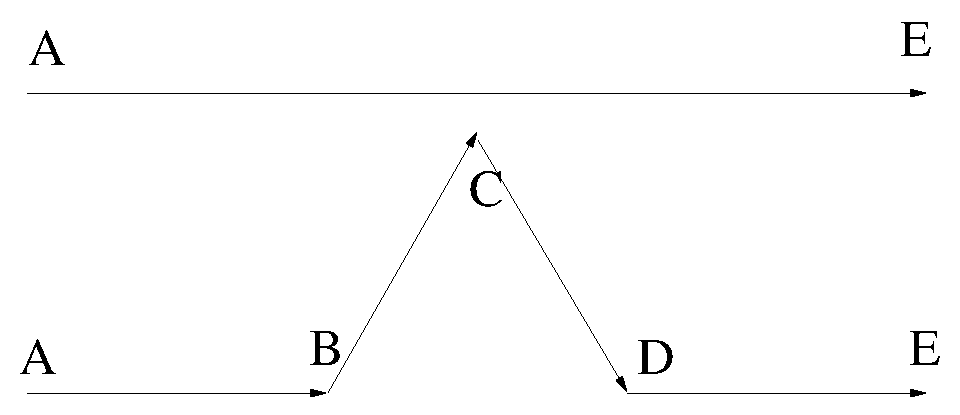
\includegraphics[width=0.4\linewidth]{vonkoch.eps}
\end{center}

Exercice 2:  \'ecrivez un algorithme pour dessiner la courbe du dragon.

\begin{center}
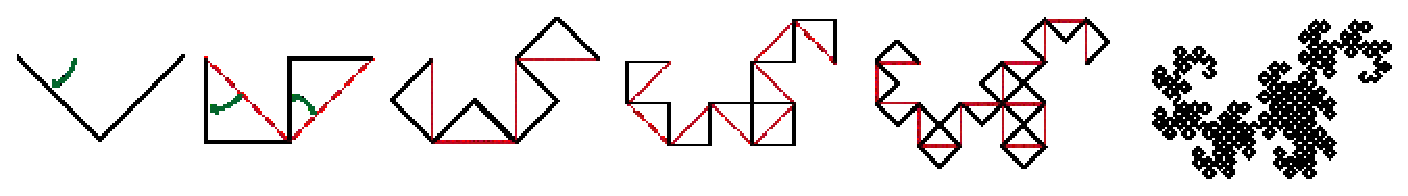
\includegraphics[width=0.8\linewidth]{dragon.eps}
\end{center}

Exercice 3: Ecrire la m\'ethode calculant 
$C(k, n)$, le nombre de fa\c{c}ons de choisir $k$ objets parmi $n$.

Exercice 4a : un arbre binaire, ordonn\'e, est donn\'e~: pour tous ses noeuds, les valeurs \'eventuelles
dans le fils gauche
sont inf\'erieures ou \'egales \`a celle du noeud, qui est inf\'erieure ou \'egale \`a toutes les 
valeurs dans le fils droit. Vous pouvez le supposer \'equilibr\'e. 
\'Ecrire un algorithme pour trouver la plus grande valeur dans l'arbre qui soit inf\'erieure
\`a un nombre donn\'e   $s$. S'il n'y en a pas (par exemple l'arbre est vide, ou toutes les valeurs dans l'arbre sont plus grandes que $s$), alors par convention votre m\'ethode rendra $\infty$.

Exercice 4b: m\^eme question que 4a, mais proposez une m\'ethode non r\'ecursive.


Exercice 5: Ecrire un tri rapide ({\it quicksort}) non r\'ecursif. C'est plus difficile~!
Vous aurez besoin d'une pile,
ou d'une autre structure d'attente.

Exercice 6: Ecrire un tri par fusion ({\it mergesort}) non r\'ecursif.

Exercice 7: Tours de Hanoi.

Exercice 8: lister les \'el\'ements d'un arbre binaire (ordonn\'e) du plus petit au plus grand.

Exercice 9 : La m\'emorisation (memoization pour les informaticiens anglosaxons), ou l'"attribut-fonction",
permettent d'optimiser les m\'ethodes r\'ecursives~; les valeurs calcul\'ees sont stock\'ees 
dans une table de hachage, ou attach\'ees en attribut sur les  donn\'ees pour la m\'ethode
de l'"attribut-fonction" (cette derni\`ere est utilisable quand 
la fonction ne prend qu'un seul param\`etre). Il est aussi possible
d'utiliser des pointeurs faibles (si le langage le permet)~: cela permet au 
gestionnaire de m\'emoire (le {\it garbage collector}) de r\'ecup\'erer 
l'espace m\'emoire occup\'e par des donn\'ees
qui n'ont pas \'et\'e utilis\'ees depuis "longtemps". Cette m\'ethode est 
int\'er\'essante dans les cas de r\'ecursion "tordue". Re-\'ecrivez l'algorithme
na\"if pour calculer Fibonacci avec cette m'ethode; que devient la complexit\'e~? 
Dans le cas g\'en\'eral (pas Fibonacci), pourquoi conseille-t-on
d'utiliser une table de hachage, et pas un tableau~? 

Exercice 10. La r\'ecursion permet de d\'efinir des fonctions de $\N$ vers $\N$ qui croissent tr\`es rapidement. La fonction d'Ackermann, ou la fonction de Kozen, en sont deux exemples.
La fonction de Kozen est d\'efinie par~: $K_0(x)=x+1, K_{n+1}(x)=K_n^{(x)}(x)$, o\`u
la notation $f^{(k)}$ signifie que $f$ est appliqu\'ee $k$ fois~: $f^{(0)}(x)=x, f^{(1)}(x)=f(x), f^{(2)}(x)=f( f( x)), f^{(3)}(x)=f( f( f( x)))$. Prouvez que $K_1(x)=2x$, que $K_2(x)=x2^x$. Calculez $K_3(2), K_3(3)$. 
Il est possible de d\'efinir des fonctions encore pire~: $G_0(x)=x+1, G_{n+1}(x)=G_n^{(G_n(x))}(x)$~: tentez de calculer $G_3(1)$ 
Ces exemples montrent que certaines fonctions r\'ecursives (donc parfaitement d\'efinies) sont incalculables en pratique.



\end{document}
\newpage

Exercice 10. Fermat a utilis\'e un concept tr\`es similaire  de r\'ecursion
pour ses preuves; pour prouver
qu'il n'existe pas d'entiers avec telle propri\'et\'e, il supposait qu'il en existe,
consid\'erait les plus petits de ces entiers, puis  il en d\'eduisait des entiers plus petits ayant
la m\^eme propri\'et\'e~: d'o\`u une contradiction. Voici 
un exemple de preuve \`a la Fermat.

Il n'existe pas de pentagone r\'egulier avec des sommets \`a coordonn\'ees enti\`eres.
Sinon soit $P_0, P_1, P_2, P_3, P_4$ un tel pentagone. Alors $P_i'= P_i+ \overrightarrow{P_{i+1}P_{i+2}}$
est aussi \`a coordonn\'ees enti\`eres (prendre les indices modulo 5), et strictement
plus petit que le pentagone  initial suppos\'e \^etre le plus petit: $P_0, P_1, P_2, P_3, P_4$.

Pourquoi cela ne marche pas avec l'hexagone r\'egulier~? avec le triangle \'equilat\'eral~? 

En fait il existe des triangles \'equilat\'eraux (et donc des hexagones r\'eguliers) entiers~:
consid\'erez sur le cube unit\'e les 3 diagonales de trois faces incidentes \`a un m\^eme sommet.
\end{document}
